\documentclass[12pt,letterpaper]{article}

\usepackage{tikz}
\usetikzlibrary{shapes}

\usepackage{amssymb,amsmath,amsthm}
\usepackage{enumerate}
\usepackage[margin=1.25in]{geometry}
\usepackage{graphicx,ctable,booktabs}
\usepackage{fancyhdr}
\usepackage[utf8]{inputenc}
\usepackage{gensymb}
\usepackage{wrapfig}

\makeatletter
\newenvironment{problem}{\@startsection
       {section}
       {1}
       {-.2em}
       {-3.5ex plus -1ex minus -.2ex}
       {2.3ex plus .2ex}
       {\pagebreak[3]
       \large\bf\noindent{Problem }
       }
       }
\makeatother

\title{Angles}
\author{Name: \underline{\hspace{5cm}}}
\date{October 3, 2015}

\pagestyle{fancy}
\lhead{Angles}
\chead{}
\rhead{\thepage}
\lfoot{\small\scshape Grade 4 Olympic Math}
\cfoot{}
\rfoot{}
\renewcommand{\headrulewidth}{.3pt}
\renewcommand{\footrulewidth}{.3pt}
\setlength\voffset{-0.25in}
\setlength\textheight{648pt}
\setlength\headheight{15pt}

\begin{document}

\maketitle

\thispagestyle{empty}

\begin{problem}{Acute, Right, Obtuse}
 Circle the correct class of each angle.

 \begin{itemize}
  \item $123\degree$ \hfill Acute~~Right~~Obtuse
  \item $62\degree$ \hfill Acute~~Right~~Obtuse
  \item $90\degree$ \hfill Acute~~Right~~Obtuse
  \item $41\degree$ \hfill Acute~~Right~~Obtuse
 \end{itemize}
\end{problem}

\begin{problem}{Angle sum}
 \begin{itemize}
  \item The sum of an acute angle and a right angle is:
        \hfill Acute~~Right~~Obtuse
  \item Half of a right angle is:
        \hfill Acute~~Right~~Obtuse
 \end{itemize}


\end{problem}

\begin{problem}{Complementary angles}
 Complementary angles sum to $90\degree$ and supplementary angles sum to
 $180\degree$. Find the complementary and supplementary angles for each of the
 following.

 \begin{itemize}
  \item $81\degree$ \hfill Complementary: \underline{\hspace{3em}}
  Supplementary: \underline{\hspace{3em}}
  \item $18\degree$ \hfill Complementary: \underline{\hspace{3em}}
  Supplementary: \underline{\hspace{3em}}
 \end{itemize}

\end{problem}

\begin{problem}{Triangle angle sum}
 The sum of the angles of a triangle is $180\degree$.
 Two of the angles measure $25\degree$ and $140\degree$.
 What does the third angle measure?
\end{problem}

\begin{problem}{Supplementary}
 Two angles are supplementary. One is $20\degree$ greater
 than the other. Find both angles.
\end{problem}

\begin{problem}{Challenge}

\begin{wrapfigure}{r}{0pt}
 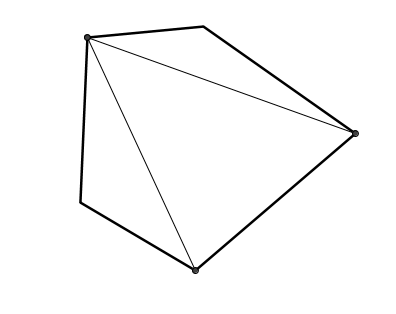
\includegraphics[width=10em]{pentagon.png}
\end{wrapfigure}

The sum of the interior angles of a triangle is $180\degree$.

\begin{enumerate}
 \item What is the sum of interior angles of a rectangle?
 \item Use the picture to show that the sum of interior angles of any pentagon
 is $540\degree$.
 \item Draw an octagon (eight-sided shape). What is the sum of its interior
 angles?
 \item When one side is added to a shape (for example, changing a triangle [$3$]
 to a quadrilateral [$4$]), by how much does the angle sum change? Why?
\end{enumerate}

\end{problem}

\end{document}\grid
